%%%%%%%%%%%%%%%%%%%%%%%%%%%%%%%%%%%%%%%%%%%%%%%%%%%%%%%%%%%%%%%%%%%%%%%%%%%%%%%%%%%%%%%%%%%%%%%%%%%%%%%%%%%%%%%%%%%%%%%%%%%%%%%%%%%%

\chapter{Theory}
\label{cha:basic_principles}

This chapter looks at the theory behind the Spectral Modeling Synthesis (SMS) technique used to analyze the audio and synthesize the sound models, specifically for vehicle sounds. Initially, the idea behind Time Frequency Analysis is discussed, looking at how frequency content of an audio waveform can be analyzed. Thereafter, the theory behind the Synthesis of the sound models is described. Following that, energy analysis techniques, which are useful in SMS, are presented.

Spectral Modeling Synthesis is based on the Analysis/Synthesis concept. The original, time domain, audio waveform is Analyzed, and various types information, also known as model parameters, are extracted from it. This information can then be used to recreate or Synthesize back the time domain waveform.

While the SMS technique does not aim to be able to recreate mathematically equivalent sounds as the original, it does attempt to use many simplifications leveraging on human psycho-acoustical models to ignore or reduce redundant data and parameters. Hence the method aims to recreate sounds perceptually similar to the original, which bodes well with the aims of the LISTEN Project.

%%%%%%%%%%%%%%%%%%%%%%%%%%%%%%%%%%%%%%%%%%%%%%%%%%%%%%%%%%%%%%%%%%%%%%%%%%%%%%%%%%%%%%%%
\section{Time-Frequency Analysis}
\label{sec:timefreq_analysis}

The Fourier Transform is a critical signal processing operation in the field of acoustics. The transform operation allows the analysis of frequency contents of signals, which is the basis of many acoustical method and processes. The Fourier transform however, makes a few assumptions which limit its use in many situations. For example, the signal being analyzed is assumed to be repetitive and stationary. However, many interesting acoustical waveforms are not stationary. For example, the waveforms of musical instruments are rarely stationary; they gradually increase in amplitude at the beginning and decay at the end.

Vehicle sounds, cannot be considered stationary in the long term either, as the sounds produced by the engine change as the various components of the engine rotate and move in operation. Similarly the noise generated by the tire and road interaction, is once again not stationary and changes depending on the position of the vehicle and the properties of road underneath it. To add to all this, the sounds of a passage of a vehicle can have various propagation effects, like Doppler-effect, which would cause a frequency shifting and thus making the sound even more non-stationary.

Hence, a technique needs to be used where a long audio waveform can be analyzed in short time intervals, during which the assumption of stationary-ness can be considered valid. This is the genesis of the Time-Frequency Analysis (TFA). Time-Frequency Analysis techniques are used to study the frequency content of non-stationary waveform, such that both time and frequency domain information can be extracted and considered simultaneously to some extent. There are limitation to the accuracy of the Time-Frequency Analysis techniques which is formalized by the Signal Processing analog of the Heisenberg's Inequality called Gabor limit (\cite{ref:Gabor}). The Gabor limit (see Eq. \ref{eqn:gabor_limit}) implies that product of a signal's bandwidth, and duration can not be less than one.

 \begin{equation}
\label{eqn:gabor_limit}
W_BT_D \geq 1
\end{equation}

where, $W_B$ is a measure of bandwidth (in hertz), and $T_B$ is a measure of time duration (in seconds).

There are many TFA techniques that can be used to analyze non-stationary data. Among the simplest and most straightforward is the Short Time Fourier Transform (STFT).


%%%%%%%%%%%%%%%%%%%%%%%%%%%%%%%%%%%%%%%%%%%%
\subsection{Short Time Fourier Transform Analysis}
\label{sec:stft_analysis}

The STFT technique looks at short time instants of the audio waveform that can then be assumed as stationary and used to generate frequency information by the Fourier Transform methods. This yields a complex spectrum of that short time signal. The spectrum�s magnitude and phase defines the frequency information of that short time signal, thus giving some information about the frequency content of original waveform that specific time instant.

When implementing the Fourier Transform, usually, a window function is used to scale the audio waveform being analyzed to simulate the repetitiveness of the signal. This stops the transform function from generating inexistent high frequency components in the spectrum because of the sudden change at the edge of the signal. Similar windowing has to be done when implementing the Fourier Transform part of STFT.

However, since the original waveform is being split into multiple short time instance waveforms, the windowing functions can also cause any information or local fluctuations (higher frequency components) at the edge of the window to be scaled down and hence lost in the analysis. So, to generate the STFT for a long waveform, the sliding window technique is used to ensure no information is lost at the edges of the short time instant waveforms.


%%%%%%%%%%%%%%%%%%%%%%%%%%%%%%%%%%%%%%%%%%%%
\subsubsection{Sliding Window Technique}
\label{sec:sliding_window}

In Sliding Window Technique, the windowing function is applied to a specific part of the signal thus selecting that short time instant, also known as a frame, to be analyzed. Once that analysis is done, the window is slide (moved to a different time index of the signal) to be applied to another section of the signal. The Fourier Transform analysis of such a windowed frame can be considered to give the frequency content of the frame of the signal centred at the centre of the section of the original waveform that was considered by the sliding window.

The number of temporal indices between the two subsequent locations where the window is applied is called �hop length�, $M$. The hop length is a measure of the temporal resolution of the analysis. The smaller the hop length, the closer the time instances of subsequent analysis locations. If the hop length is smaller than the length of the window, $N$, there will be an overlap in the audio signal analyzed in the subsequent Fourier Transforms. In cases where the hop length, $M$ is close to the half of the length of the window $N$, the audio signal at the edge of one window, will end up near the centre of the window in the subsequent analysis, hence ensuring that all the information is captured in one of the frames of STFT. Figure \ref{fig:stftdiagram} shows an example sliding window over an arbitrary audio waveform. The various overlapping windows indicated are the sections of the audio waveform that are analyzed during each hop.

\begin{figure}
\begin{center}
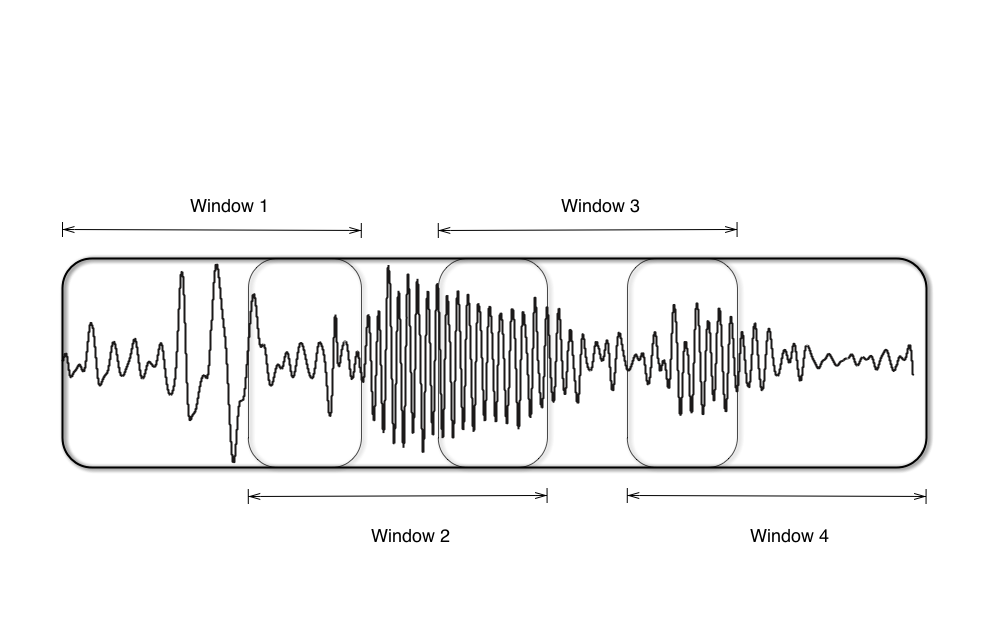
\includegraphics[height=9.20cm]{../images/STFTdiagram.png}
\caption{Diagram of a Sliding Window Analysis over an audio waveform.}
\label{fig:stftdiagram}
\end{center}
\end{figure}


Eq.\ref{eqn:slid_wind} gives a discrete-time representation of a STFT, with $x[n]$ being the audio signal being analyzed, $w[n]$ being the sliding window used to limit the analysis to the time instant under consideration. The exponential term implements the Fourier Transform.

\begin{equation}
\label{eqn:slid_wind}
STFT\{x[n]\} \equiv  X[m,\omega] = \sum_{n = -\infty}^{\infty}x[n]w[n-m]e^{-j\omega n}
\end{equation}

This expression gives the frequency content $X[w]$ at each time instant, defined by the index $m$ of the audio signal.

A spectrogram is a 3-dimensional representation of a STFT analysis. The MATLAB $spectrogram$ function allows one to visualize the frequency content of the signal at each time interval, based on the parameter supplied.


%%%%%%%%%%%%%%%%%%%%%%%%%%%%%%%%%%%%%%%%%%%%
\subsection{Overlap and Add Synthesis}
\label{sec:OAASynthesis}

The STFT technique is used to analyze the frequency content of a time domain waveform. However, due the use of the Sliding Window Technique, while the frequency information at a certain given time instant is captured, there is no simple way to recompose this information back into the original time domain signal.

The Fourier Transform converts a time domain waveform into a frequency domain spectrum. The Inverse Fourier Transform allows the conversion of a frequency domain spectrum into a time domain signal. While these operation are unitary, the overlapping of the analyzed signal caused by the sliding window technique with a hop length less than the window length, does not allow the time domain signal generated by the inverse Fourier Transform to be simply concatenated.

If the two successive STFT analyzed frames undergoes an Inverse Fourier Transform, the overlapped portions of the two successive time domain signals should have the same values, and hence one of them can be ignored allowing concatenation of the rest of the re-transformed time domain signal. However, if some processing and operations are done on the analyzed frequency content, the overlapped portion might not be the same, and hence needs to be considered.

A technique called Overlap and Add is used to recreate the time domain signal. This technique overlaps the successive time domain signal data generated by the Inverse Fourier Transform, scales them by a windowing function and adds the two waveforms. This allows the information from both the successive time domain signals to be captured and yet ensures that the total magnitude of the resultant signal from the addition does not exceed the maximum. This is similar to taking the weighted average of the contribution from each of the time domain signals, and thus captures relevant information.

%%%%%%%%%%%%%%%%%%%%%%%%%%%%%%%%%%%%%%%%%%%%
\subsubsection{Constant Overlap and Add (COLA)}
\label{sec:COLA}

While using an Overlap and Add technique for the synthesis of the STFT analyzed audio, one also needs to ensure that the addition process does not affect the signal. The window and overlap ratio need to be constrained to ensure that time domain signal after the, sliding window analysis and overlap-add re-composition, is the same as the original time domain signal.

Considering a sequence of windowed short time instant signals, $x_m(n)$, which are generated from an original signal $x(n)$ using a sliding window $w(n)$ with hop length $R$, we can enforce the re-composition using overlap and add operation, $x_r(n)$ on that sequence to yield back the original signal $x(n)$.

From Eq.\ref{eqn:colaEqn}-\ref{eqn:colaEqnFin}, this constraint can be met if the sum of the window magnitudes equals to 1. This is the Constant Overlap and Add (COLA) constraint. Various combinations of window and overlap ratios meet this constraint. Table \ref{tab:colaWind} gives an example of few such combinations, where $R$ is the hop length and $M$ is the window length.

\begin{align}
\label{eqn:colaEqn}
x_r(n) & = \sum_{m=-\infty}^{\infty} x_m(n)\nonumber \\
       & = \sum_{m=-\infty}^{\infty} x(n)w(n-mR) \nonumber \\
       & = x(n)\sum_{m=-\infty}^{\infty}w(n-mR)
\intertext{Thus, to recompose the original signal after the Overlap and Add,}
x_r(n) = x_(n)\nonumber \\
\intertext{Hence}
x(n) = x(n)\sum_{m=-\infty}^{\infty}w(n-mR) \nonumber
\label{eqn:colaEqnFin}
\\ 1 = \sum w(n-mR)
\end{align}

\begin{table}[h]
\begin{center}
\begin{tabular}{ | l | l |  }
    \hline
       Window Type & Conditions \\ \hline \hline
       Rectangular  & $R=M; R=\frac{M}{2}$\\
       Bartlett  & $R=\frac{M}{2}$\\
       Hamming & $R=\frac{M}{2}; R=\frac{M}{4}$ \\ \hline
       Hann & $R=\frac{M}{2}$
  \end{tabular}
  \caption{Combinations of window types and overlap ratio which ensure COLA.}
  \label{tab:colaWind}
   \end{center}
  \end{table}

Ensuring COLA allows the use of the sliding window technique for STFT analysis as well as the Overlap and Add technique for synthesis without loosing any information.

%%%%%%%%%%%%%%%%%%%%%%%%%%%%%%%%%%%%%%%%%%%%
\subsection{Spectral Modeling}


With COLA, the STFT technique for Analysis and Overlap and Add technique for Synthesis, make up a chain of processes that allow exact synthesis of the original audio. This is the foundation of Spectral Modeling. With the ability to analyze the frequency content of audio waveform and then synthesize it from the analyzed frequency content, the frequency domain information can be used to extract data and parameters.

The Spectral Modeling synthesis technique models the time-varying spectra of an audio waveform as a collection of sinusoids and a time-varying noise component. This method is based on the Additive synthesis \cite{ref:addSynth} technique. The Additive synthesis technique assumes that any periodic waveform can be created by the addition of a set of sinusoids at various amplitudes and harmonic frequencies. This simple model however breaks down in the case of many natural sounds, where not all of the critical aspects of the sounds are tonal in nature. A sum of sinusoids is capable of modeling tonal sounds very well, however, with less deterministic sounds, like noisy vehicle sounds, or breath noises in wind instruments, the Additive Synthesis model is not able to capture the energy in the noisy portion of the original waveform, as a noisy signal cannot be described by a sinusoid, but instead is defined by a probabilistic power spectral density.

The SMS technique, separates the audio waveform into; the deterministic component, which can be defined by a narrow band quasi-sinusoidal waveform (with time-varying amplitude and frequency); and the stochastic part, which is modeled by a time varying envelope function defining the amplitude of the probability density of the signal.

The separation of the two types of signal contents allows for easy modeling and data compression of the signal, and also a simpler method to manipulate and process the parameters.

Mathematically, this approach can be modeled as shown in Eq.\ref{eqn:stocDet} degenerating the waveform into a sum of sinusoidal signals and an error signal which is the noisy component. Here $s(t)$ is the original audio signal, $A_i$ is the amplitude of each of the $N$ sinusoid components, $\omega_i$ is the frequency of each of the sinusoids, and $e(t)$ is the error signal which is modeled as the stochastic part.

\begin{equation}
\label{eqn:stocDet}
s(t) = \sum_{i = 1}^{N} \left(A_i \times \cos(\omega_i \times t)\right) + e(t)
\end{equation}

The model assumes that all the sinusoids are stable, and the amplitude and frequency only changes gradually, and within a small range, in comparison to the frequency of analysis instances. Such sinusoids usually make up the tonal sounds from musical instruments, and support musical processes of vibrato, and pitch bending, where sinusoidal signal gradually change their frequency within a small range. Such effects are also noticeable in environmental sounds like roughness of engine noises, and the pitch shift caused by the Doppler effect. Hence, this assumption holds well in the case of sounds being modeled for the LISTEN Project.

\begin{figure}
\begin{center}
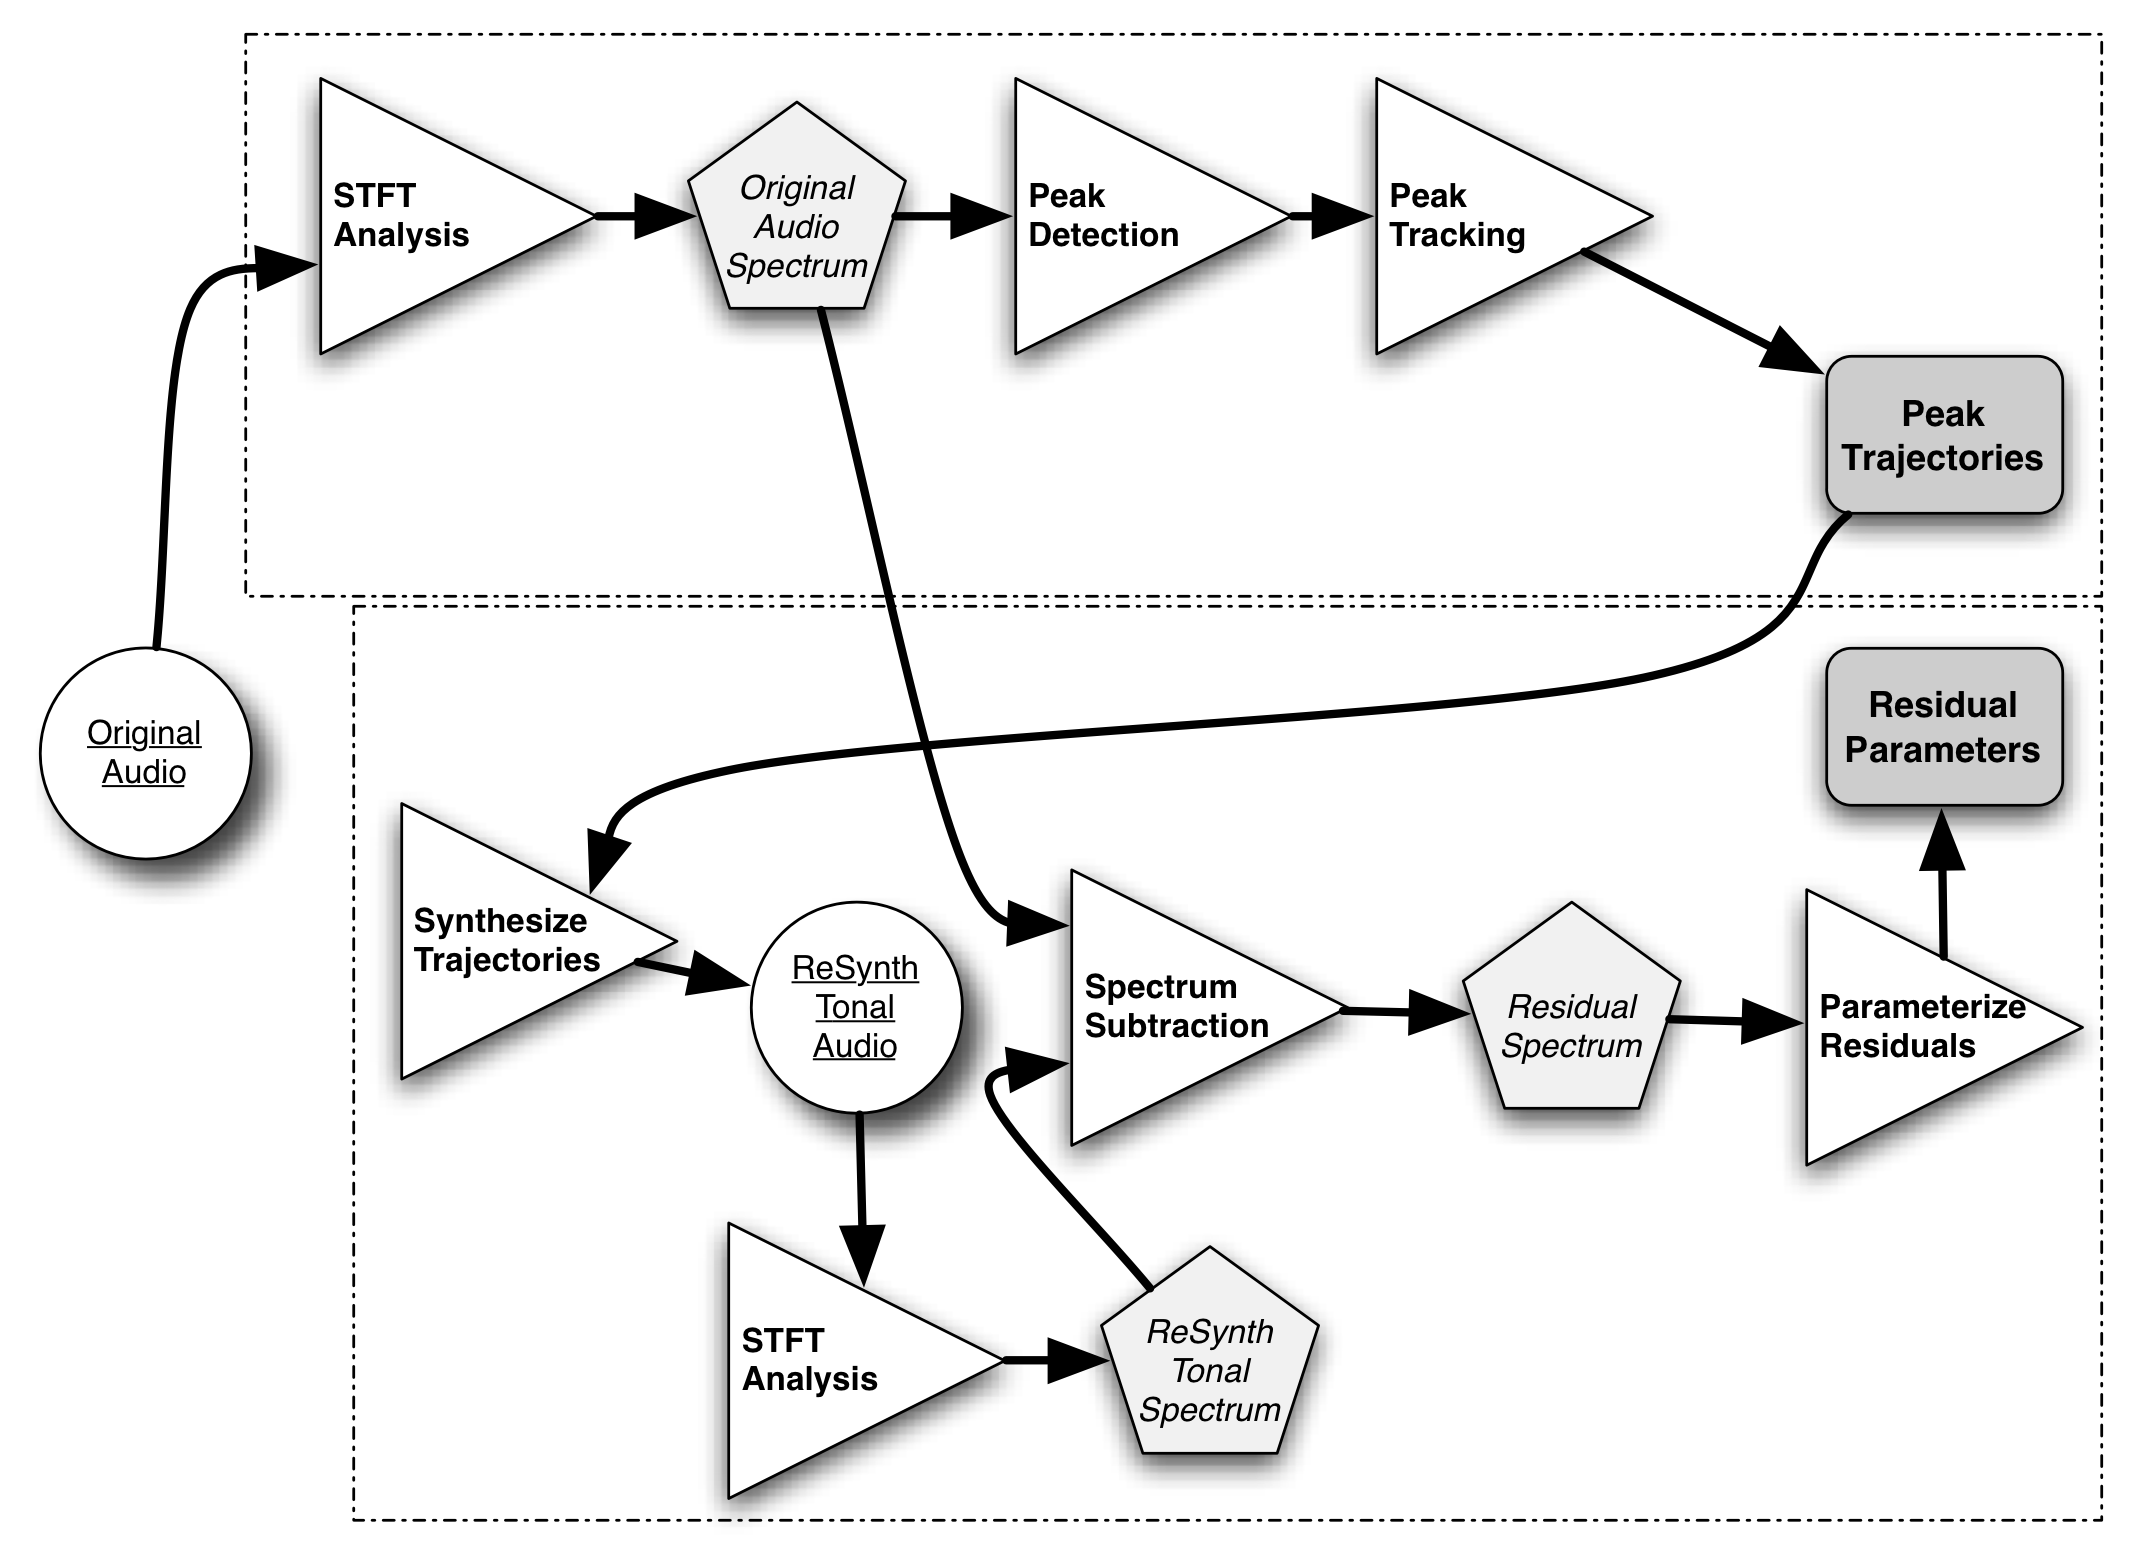
\includegraphics[height=8.7cm]{../images/BlockDiagramAnalysis.png}
\caption{Block diagram of the analysis section of the Spectral Modeling Synthesis Technique.}
\label{fig:smsAnalysisBlock}
\end{center}
\end{figure}

Figure \ref{fig:smsAnalysisBlock} shows a block diagram of the analysis part of the Spectral Modeling Synthesis technique. The analysis part consists of a calculation of a series of spectra based on the sliding window technique and STFT as discussed in section \ref{sec:stft_analysis}. The spectral information from that operation is used to detect quasi-sinusoidal components in the sound. The spectral content that can not be modeled as sinusoidal components is then captured as a residue and modeled as noise.


%%%%%%%%%%%%%%%%%%%%%%%%%%%%%%%%%%%%%%%%%%%%
\subsection{Peak Detection and Tracking}

%%%%%%%%%%%%%%%%%%%%%%%%%%%%%%%%%%%%%%%%%%%%
\subsubsection{Peak Detection}
\label{sec:peakDet}

A Fourier Transform of an infinitely long sinusoid of a certain frequency yields a Dirac Delta function. In the digital domain, an impulse at the frequency of the sinusoid is seen in the Discrete Fourier Transform of such a sinusoidal signal. Performing STFT analysis of a long waveform, assuming that it is made of gradually changing sinusoidal components, implies that within each frame analyzed by the STFT process the amplitudes and frequencies of each sinusoid are constant, and can be detected from the peaks in spectral waveform. Hence, peak detection is critical in capturing the sinusoidal components in the SMS method.

A peak is defined as a local maximum in the magnitude of the spectrum. Thus, a simple maximum detection algorithm can be used to detect the peaks. However, the nature of the analysis technique makes the peak detection more complicated than just a search for change of gradient of the magnitude spectrum from positive to negative.

Firstly, since the Discrete Fourier Transform (DFT) is used in STFT, the frequency information in the spectrum is also discretized, it is harder to guess the exact maxima of the peak. While a change of gradient, as described in Eq.\ref{eqn:changeOfGrad} does indicate a peak in the vicinity of the discrete points, the data needs to be interpolated to find the exact location (which could be in-between two of the discrete frequency points generated by the DFT) of the peak. A simple way to improve the accuracy of this is to add zero padding when doing the DFT. This causes the difference between discrete frequency indices to reduce, thus giving a better resolution of magnitude, allowing for more accurate peak detection.

\begin{equation}
\label{eqn:changeOfGrad}
  a_n = x[n]; f_n = f[n]; \forall n \in \left\{ \dot{x}[n-1] > 0  \text{ and } \dot{x}[n] \le 0 \right\}\\
\end{equation}

where $a_n$ is the amplitude of the peak and $f_n$ is the frequency of the peak, defined at all points in the spectrum where the gradient changes.

However, even with zero padding, it�s rare to have the one of the discrete frequency indices to fall exactly at the peak frequency, hence an interpolation still needs to be done to guess the exact maxima of the peak. The shape of the peak is dependent on the analysis window type used in the sliding window technique. Eq.\ref{eqn:windFFT} shows interaction of the window function with the sinusoid, giving the final spectrum a shape of the Fourier Transform of the window itself.

\begin{equation}
\label{eqn:windFFT}
FFT(x[n] \times w[n-M]) = W(k-w_0)
\end{equation}

Knowing the shape of the window spectrum, we can interpolate the DFT data to fit that function. An analytical expression of the shape of the window spectrum is needed for such interpolation, which might not be possible for some window types.

However, a good trade off can be achieved by doing a simple quadratic interpolation in the decibels (dB) scale. While this yields an accurate representation of the spectrum function in case of the Gaussian window \cite{ref:sms}, a quadratic function can also be a good second degree polynomial estimation of many of the peak spectrum functions, and hence is good enough to estimate the maxima in many cases.

Secondly, the perceptual importance of peaks also needs to be taken into account. Auditory Masking effect makes tones close in frequency to other tones or noise less audible. Thus, in the peak detection stage, it is not necessary to detect all peaks, but instead consider the peaks in the context of the surrounding peaks, picking only those that would be distinguishable to a human hearing.

Finally, in the case of two sinusoid at frequencies very close to each other, the peaks can overlap and make it harder to detect the separate peaks and hence can make the interpolation for the estimation of the spectrum maxima harder as well.

\subsubsection{Differential Peak Amplitude Calculation}

A more accurate method for detection of peaks was introduced by Desainte and Marchand \cite{ref:accuratePeak}. This method uses a DFT of the 1st derivative of the windowed audio signal to calculate a more accurate amplitude and frequency of the peak. Desainte and Marchand show that the ratio of the DFT of the windowed audio signal and the DFT of the 1st derivative of the windowed audio signal are related by a factor of the frequency of the peak as shown in Eq.\ref{eqn:accuratePeak}. This can also be seen from the purely complex Fourier transform, also know as the '$j\omega$ transforms' that is commonly used in physical Acoustics as the $j\omega$ factor relating the Fourier representation of the time domain signal and its first derivative.


\begin{equation}
\label{eqn:accuratePeak}
f_{p} = \frac{1}{\pi}\frac{DFT^1(f_p)}{DFT(f_p)}.
\end{equation}

Using this method a more accurate estimate of the peak frequency can be detected, without the need to interpolate over the window spectrum function. This method also allows the calculation of accurate amplitude with the knowledge of a continuous spectrum $W$ of the analysis window used for the DFT. Eq.\ref{eqn:accuratePeakAmp} can be used for that calculation.

\begin{equation}
\label{eqn:accuratePeakAmp}
a_p = \frac{a_p^0}{W|f_p-f_p^0|}
\end{equation}

where, $a_p^0$ is an estimate peak amplitude, $f_p^0$ is the frequency of the estimated peak amplitude, $f_p$ is the accurate frequency of the peak, based on Eq.\ref{eqn:accuratePeak}. The required estimates can be seeded from the maximum detection method described in Section \ref{sec:peakDet}.

Another benefit of this technique is that it removes the effect of the analysis window on the amplitude of the peak. Whereas in a normal gradient based peak detection technique effect of the analysis window on the amplitude of the peak has to be done separately as explained in Section \ref{sec:peak_amp_cacl}.

\subsubsection{Peak Tracking}
\label{sec:peakTrack}

While peak detection gives a set of possible sinusoids corresponding to each peak in each frame, the individual peaks need to be analyzed to find patterns of series of peaks which may form a quasi-sinusoidal component. This peak tracking or peak continuation as defined by Serra \cite{ref:sms}, tries to find gradually changing tonal components by looking at peaks in each individual time instant and finding peaks that form a good continuation of the sinusoids in the next time instant.

The technique described by Serra uses the idea of a frequency guide, which is advanced every time instant depending on the peaks detected in the frame from that specific instant, forming a trajectory for the sinusoid. The guide helps to smoothly influence the frequency and the amplitude of the sinusoid to generate a gradually changing sinusoid.

The gradual start and end of the guides is enforced in this technique, along with the ability of these guides to remain dormant. A dormant guide may not track any peaks for certain time instants, but may continue after some time instances. This is provisioned to allow scenarios when noise levels go above the amplitude of the sinusoid and it can�t be detected. This is typical in sounds with high noise levels, like outdoor sounds. In such scenarios, the guide can pause and start tracking the sinusoid when an appropriate peak is detected in the future time instants.

In the entire process of peak tracking and continuation, the phase information is completely disregarded. When considering sinusoids, only the starting phase of the sinusoids is important as rest of the samples of the sinusoid have a phase that changes regularly with time based on the frequency of the sinusoid. Hence all the phase information can be conveniently ignored in the deterministic analysis and reconstructed during the synthesis by just knowing the initial phase of each of the sinusoid.

In Serra's design, the initial phase of each sinusoid was assumed to be 0. The main motivation for that is the very small number of guides and sinusoids that are needed to be tracked in the musical sounds, and so interaction between tones at slightly different phases would not affect the synthesized sound as much perceptually. This assumption may not hold for other types of sounds.

The peak continuation technique allows a series of peaks to be curated which can define one of the tonal components of the sounds in the SMS model. The amplitude and the frequency of each of these trajectories form the set of parameters that define the deterministic part of SMS model. These trajectories can be used to generate individual sinusoids, which can then be added to generate the final tonal component of the sound. While this modeled tonal component might not be mathematically equal to the actual tonal component in the original sound due to inaccuracies in peak detection and perception based simplifications, the aim of the model is to be able to generate sound which are perceptually similar, which this sinusoidal modeling accomplishes.

%%%%%%%%%%%%%%%%%%%%%%%%%%%%%%%%%%%%%%%%%%%%
\subsection{Residuals and Parametrization}


%%%%%%%%%%%%%%%%%%%%%%%%%%%%%%%%%%%%%%%%%%%%
\subsubsection{Residual Calculation}
\label{sec:residualcalc}


Peak detection and peak tracking yields the information about the tonal components of the sound. In the SMS technique a part of the sound is assumed to be of tonal and noisy (quasi-stochastic). Having modeled the tonal component, the noisy component can be computed by just removing the tonal components from the original sound. Hence, Serra refers to the noisy component as the residual. This step needs a little elaboration.

The removal of the modeled tonal component can either be done in time domain, waveform subtraction, or in frequency domain, spectral subtraction. Both methods have to ensure that no information is lost during the subtraction process.

The time domain method only works if the phases of the tonal components are known with accuracy. However, in the peak tracking and continuation method, the phase of the tonal component is lost as only the magnitude of the peaks in considered. And since the modeled tonal components are not analytically similar to the tonal component of the original sound, a time domain subtraction would not work in this case.

The time domain method, can be described by Eq.\ref{eqn:timeDomainSub},

\begin{equation}
\label{eqn:timeDomainSub}
r[n] = x[n] - x_r[n]
\end{equation}

where, $x_r[n]$ is the synthesized deterministic signal.

The frequency domain method also faces the same issue with the lack of the phase data of the tonal spectrum. Very little information of the tonal spectrum is known, since only the amplitude and frequency of the maxima of the peaks of the tonal spectrum are captured during peak tracking. The rest of the spectral amplitudes have to be generated, and so does phase information of the entire tonal spectrum.

The frequency domain method, can be described by Eq. \ref{eqn:freqDomainSub},

\begin{equation}
R_i[n] = \left\{
  \begin{aligned}
  & X_i[n] - X_{i,r}[n] & \quad \forall \text{ n where }X_i[n] > X_{i,r}[n]  \\
  & 0 & \quad \forall \text{ n where } X_i[n] \le X_{i,r}[n]
  \end{aligned}
\right.
\label{eqn:freqDomainSub}
\end{equation}

where, $X_{i r}$ is the $i$-th frame of the spectrum of the synthesized deterministic signal.

The relationship between the peak maxima and amplitude of the spectrum around the peak depends on the windowing function. But along with that, the interaction of the various peak functions make generation of the peak amplitudes in the frequency domain based on the peak maxima values a complicated task. Serra instead recommends synthesizing the trajectories in time domain (as described in Section \ref{sec:tonal_synth}) and then reanalyzing them using the STFT method to yield a complete tonal spectrum. This not only models the interaction of the peak amplitudes but also ensures that any other processing done during the Synthesis process is captured and used in calculating of the residual component. This way the magnitude spectra of the tonal and original signal can be subtracted at each time instant to yield the residual magnitude spectra. While this technique consumes more steps of calculations and is repetitive, the benefits of frequency domain subtractions make it a worthwhile choice.

The lack of initial phase information of the tonal component is still an issue in spectral subtraction method. However, since the residual component is assumed to be noise with a quasi-stochastic power spectral density, the phase information is redundant in the perceptual representation of the sound. Thus, the phase information can be disregarded and generated randomly during the synthesis.

The residual calculation yields a magnitude spectrum of the residual noise for each frame of the sound. Half of this magnitude spectrum is redundant, since the the spectrum of a real signal is always mirrored. Thus, half of the spectrum can be disregarded while the other half can be further parameterized using some noise perception models.


%%%%%%%%%%%%%%%%%%%%%%%%%%%%%%%%%%%%%%%%%%%%
\subsubsection{Residual Parametrization}
\label{sec:residualparam}

The human perception of noise has been studied very well. Perception of noise in the human ear is not based on the spectral peaks like the perception of tones or even related to information in individual spectral frequencies \cite{ref:psycho}. Instead the human ear perceives noise based on the energy levels within a energy band \cite{ref:goodwin}. Thus, instead of modeling the residual magnitude spectrum using individual frequency points, it can be modeled using simpler and more compressed expressions based on energy bands. Two approaches for doing this can be considered.

Serra recommends using a envelope modeling approach. Since the individual frequency information in the magnitude spectrum is redundant, the shape of the envelope can be detected and saved in the form of a simple line-segment approximation or more complicated Linear Predictive Coding based approximation \cite{ref:lpcEnv}. The two methods have their own strength and limitations with flexibility and total captured data needed.

Another approach presented by Goodwin uses the Psycho-acoustic concept of critical bands. The human ear processes information based on overlapping frequency bands. It has been shown that within these critical bands, the actual magnitude of the spectrum at the various frequencies is not as important as the energy content within that band. Hence each band can be parameterized using the value of energy content in the band, which can be calculated as shown in Eq.\ref{eqn:resEnergyBand},

\begin{equation}
\label{eqn:resEnergyBand}
E(b) = \frac{1}{M}\sum_{k \in band b}\left|X_i[k]\right|^2
\end{equation}

$M$ is the FFT Size, $X[k]$ is the $k$th component of the FFT spectrum and $b$ is the index of the critical band being analyzed.

Either of the techniques allow the parametrization of the residual spectrum, for data compression and ease of manipulation and synthesis.

%%%%%%%%%%%%%%%%%%%%%%%%%%%%%%%%%%%%%%%%%%%%%%%%%%%%%%%%%%%%%%%%%%%%%%%%%%%%%%%%%%%%%%%%
\section{Synthesis}

With both the sinusoidal and residual components parameterized, the SMS based sound model can be synthesized to generate a perceptually similar sound to the original sound. The two components of the model can be synthesized separately and then summed to create the final sound.

%%%%%%%%%%%%%%%%%%%%%%%%%%%%%%%%%%%%%%%%%%%%
\subsection{Tonal Synthesis}
\label{sec:tonal_synth}


The Tonal Synthesis takes the set of trajectories, each being a list of amplitude and frequency pairs, that define gradually changing quasi-sinusoids. The synthesis technique generates a sinusoid for each of the trajectories and finally uses additive synthesis to sum them together to generate the time domain tonal component of the sound.

However since the sinusoidal amplitudes are only defined at the centre of the each frame, the amplitude needs to be interpolated between the two points, over a hop length, to simulate a smoothly changing sinusoid, and also to avoid clicks and other artefacts at boundaries.

The phase of the sinusoid is also required to transition smoothly between each of the frames to generate quasi-sinusoids, however since the original phase information is not captured, the instantaneous phase has to be guessed and generated based on an initial phase and instantaneous frequency of the sinusoid.

\begin{eqnarray}
\label{eqn:totalReSynthSt}
\hat{A}(m) = A^{l-1} + \frac{A^{l} - A^{l-1}}{H} m \\
\hat{\omega}(m) = \omega^{l-1} + \frac{\omega^{l}- \omega^{l-1}}{H}m\\
\hat{\theta}(m) = \theta(l-1) + \hat{\omega}(m) m
\label{eqn:totalReSynthEd}
\end{eqnarray}

Eq.\ref{eqn:totalReSynthSt}-\ref{eqn:totalReSynthEd} define the interpolation of the amplitude and phase information of a single trajectory. The instantaneous phase at each time instant is just the integral of the instantaneous frequency, which in-turn is just the linear interpolation of the frequencies of the peaks defining each frame. The amplitude at each time instant is just the linear interpolation of the amplitude of the peaks.

\begin{equation}
\label{eqn:totalReSynthFinal}
y_d(m) = \sum_{r=1}^{N}\hat{A_r}(m)\cos[\hat{\theta_r}(m)]
\end{equation}

Eq.\ref{eqn:totalReSynthFinal} defines the final synthesis equation for a single hop length, where all the trajectories defined over that hop are summed up to generate the sound for that hop. Repeating this for each hop in the sound and concatenating them generates the tonal component of the sound.

%%%%%%%%%%%%%%%%%%%%%%%%%%%%%%%%%%%%%%%%%%%%
\subsection{Residual Synthesis}

The residual component of the synthesis is modeled as parameterized magnitude envelope of the residual spectrum. To synthesize the residual component first, the parameters need to be interpolated into the complete magnitude spectrum.

If the line segment envelope method is used, then the line segments need to be interpolated to have the magnitudes at each frequency index. If the critical bands method is being used, then the square root of energy density of each band can be equally distributed among each of the frequency indices in that band, giving a step-wise estimate of the spectrum. Energy density can be defined as the energy per index in the band.

To generate a frame of time domain signal from each magnitude spectrum, the Inverse Discrete Fourier Transform (IDFT) operation can be used. For a complete and real IDFT of the spectra, phase information needs to be added to the magnitude spectra. Based on the assumption of the residual signal being pseudo-stochastic noise defined by its power spectral density, the phase information is redundant. Hence a random phase can be assigned to the magnitude spectra, and the IDFT of that will give a perceivably similar noise signal to the original residual.

\begin{equation}
\label{eqn:resSynthSpec}
Y[k] = \hat{E}[k]e^{j\Theta[k]}
\end{equation}

The interpolated magnitude spectrum can then be multiplied by a random phase spectra to form the complex residual spectra as in Eq \ref{eqn:resSynthSpec}. Where, $\hat{E}$ represents the interpolated spectral amplitude, and $\Theta$ is the a vector of random numbers. A uniform random phase which covers the entire range from $-\pi$ to $\pi$ is sufficient to generate the noise. The IDFT of the complex residual spectra yields the time domain residual noise signal as of Eq \ref{eqn:resSynthFin}.

\begin{equation}
\label{eqn:resSynthFin}
y_r(k) = \frac{1}{N} \sum_{k=-N/2}^{k=N/2-1}Y[k]e^{j\omega_k m}, m = 0,1,2,...N-1
\end{equation}

Since the residual information is captured and parameterized for each frame, the synthesis process generates the time domain residual signal for each frame. Based on the duality of the sliding window technique for analysis, which was used to generate the residual spectra in the first place, and the overlap and add technique as discussed in Section \ref{sec:OAASynthesis}, the time domain signals for each frame can be overlapped and added to generate the final synthesized residual sound.

Since, the residual being re-synthesized as been assumed as noise, the window function used in the overlap and add process must be one which preserves the perceivable characteristic of the noise, which is power. Serra recommends using a simple Hanning window, but in that case the power gain/loss of the noise as a result of the window needs to be compensated for by scaling the window. This is generally done using a factor known as the incoherent power gain which is defined as:

\begin{equation}
\label{eqn:powerGain}
G_{incoherent} = \frac{1}{N}\sum^{N}_{i=1} w[i]^2
\end{equation}

where $w[i]$ is the window function and $N$ is the window length.

With both the tonal and residual sounds being produced, they again can be summed up together to regenerate the final synthesized sound. Figure \ref{fig:smsSynthesisBlock} shows the block diagram for the synthesis section of the Spectral Modeling Synthesis technique.

\begin{figure}
\begin{center}
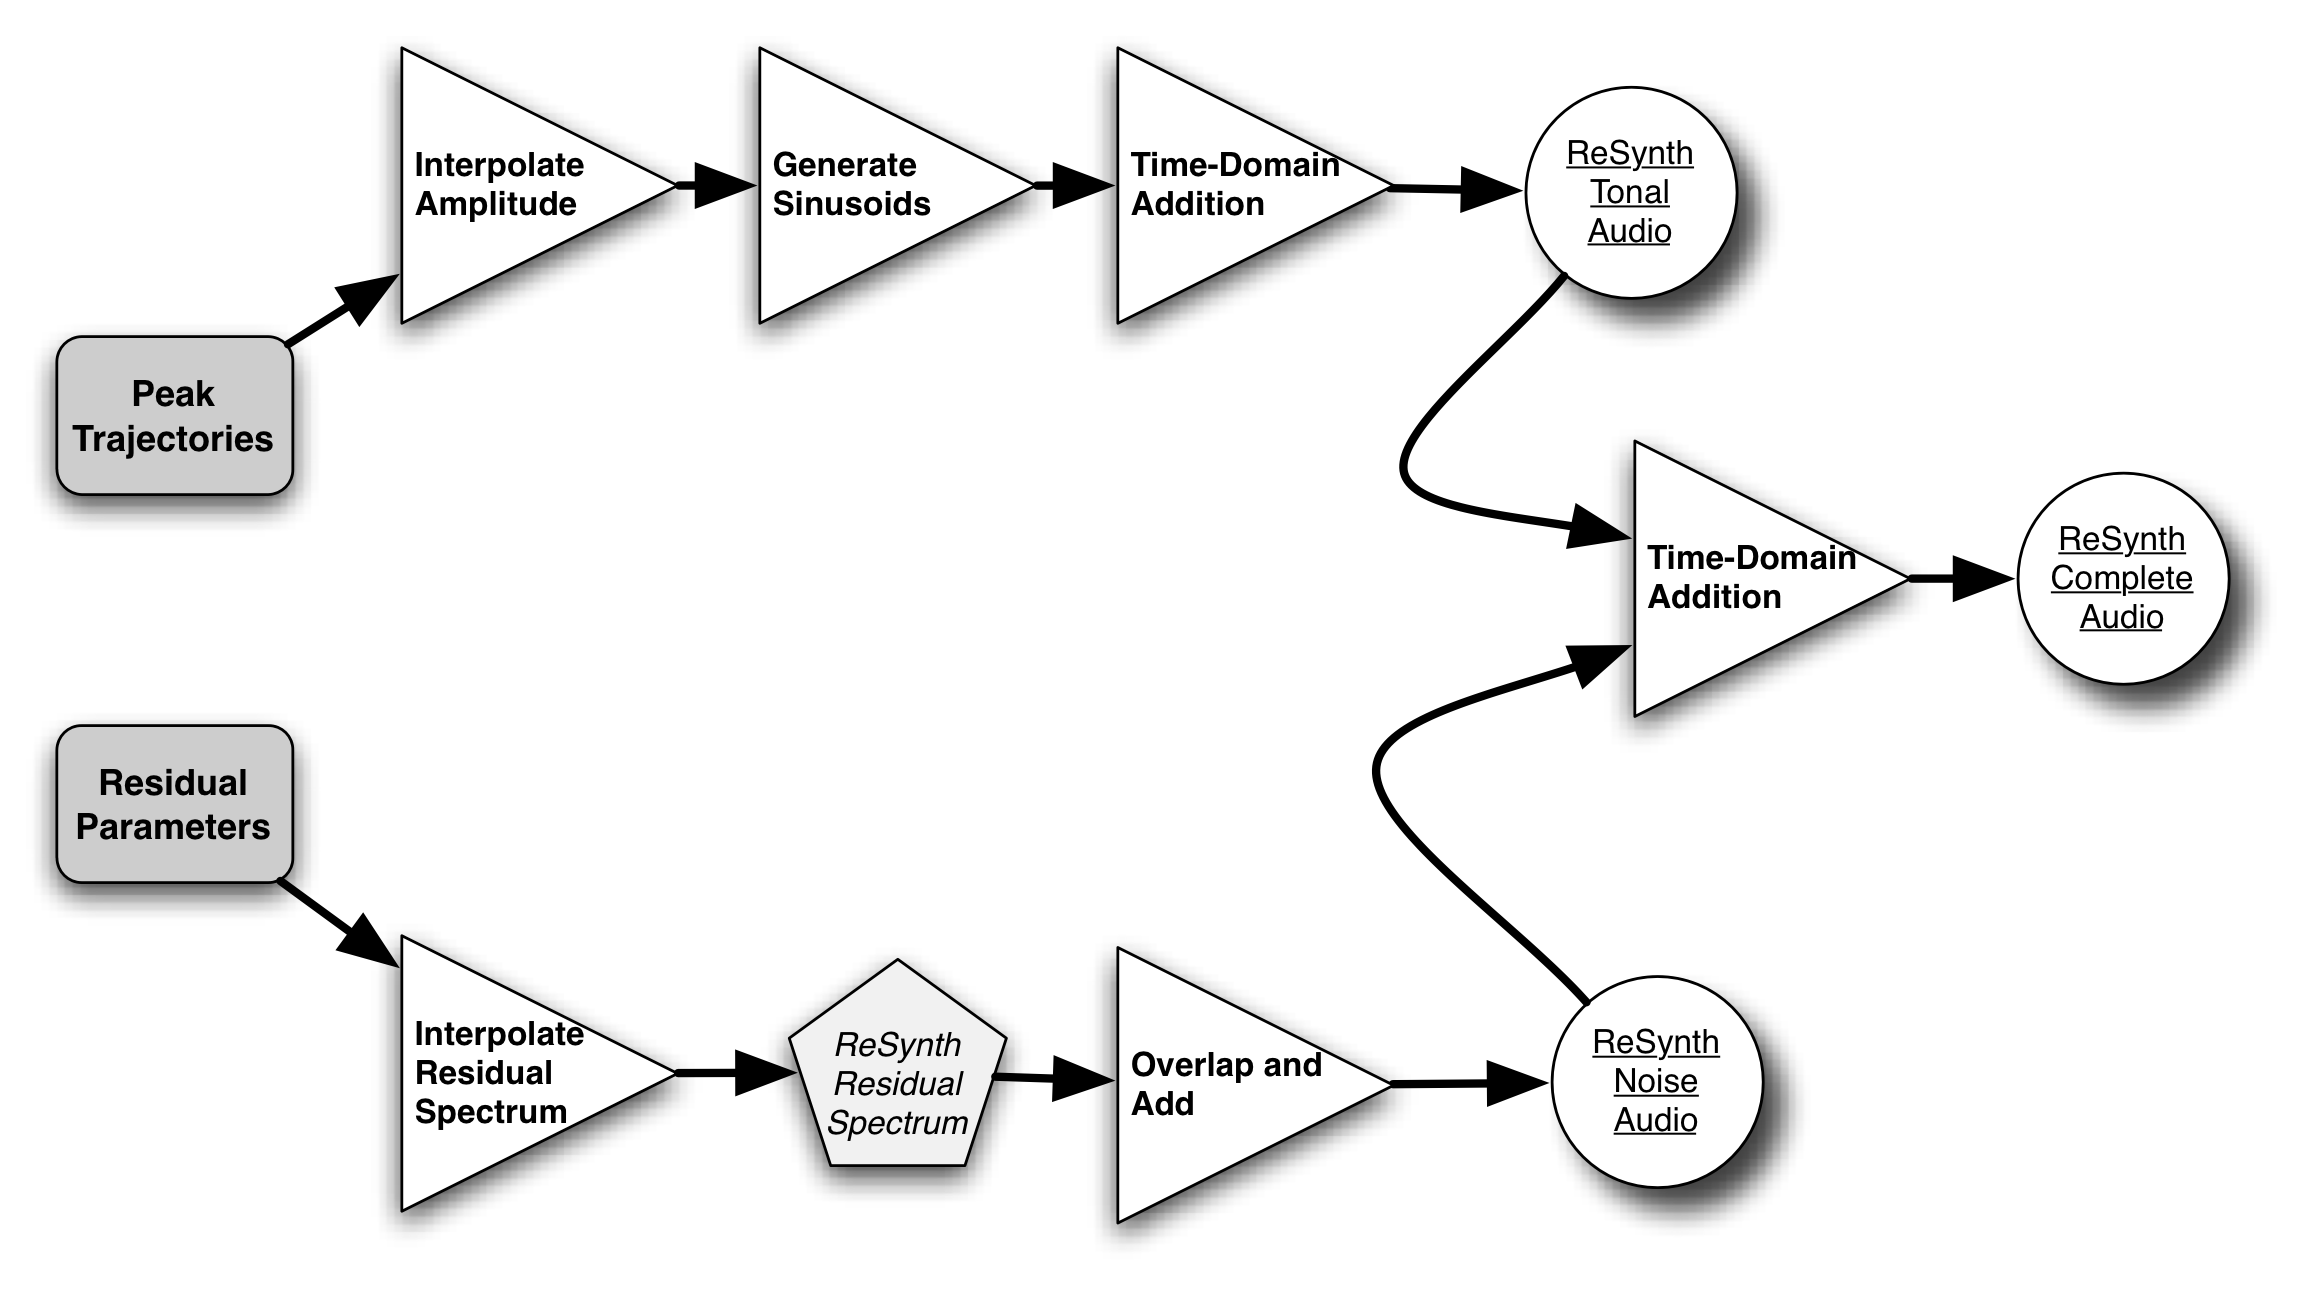
\includegraphics[height=9.0cm]{../images/BlockDiagramSynthesis.png}
\caption{Block diagram of the synthesis section of the Spectral Modeling Synthesis Technique.}
\label{fig:smsSynthesisBlock}
\end{center}
\end{figure}

%%%%%%%%%%%%%%%%%%%%%%%%%%%%%%%%%%%%%%%%%%%%%%%%%%%%%%%%%%%%%%%%%%%%%%%%%%%%%%%%%%%%%%%%
\section{Energy Analysis}
\label{sec:energy_analysis}

Another important aspect of the theory behind the Analysis/Synthesis process implements for this Thesis is the Energy Analysis. The SMS technique relies of splitting the given sound into two parts and then recombining them during synthesis. Thus, ensuring that the energy (or power) of the signal is being modeled accurately and tracking the flow of the energy between the various components is critical for such an Analysis/Synthesis process to work effectively.

%%%%%%%%%%%%%%%%%%%%%%%%%%%%%%%%%%%%%%%%%%%%
\subsection{Energy in Transform Domain}


Since the SMS technique uses transitions many a times between times and frequency domains using Fourier Transforms, it is important to understand the calculation of energy in both domains. Parseval�s theorem, Eq \ref{eqn:parsevals}, defines the relationship between the energy of time and frequency domain discrete signals.

\begin{equation}
\label{eqn:parsevals}
 E = \sum_{n=0}^{n=N-1}|x[n]|^2 = \frac{1}{N} \sum_{k=0}^{k=N-1}|X[k]|^2
\end{equation}

It is important to note the normalization factor of 1/N on frequency domain summation. This normalization factor is also important when dealing with simple Fourier Transforms. A normalized Fourier transform of a sinusoid yields a magnitude spectrum which has an amplitude equal to the amplitude of the sinusoid. This is critical for peak detection in tonal synthesis where the amplitude of the peak is used as the amplitude of the sinusoid.

%%%%%%%%%%%%%%%%%%%%%%%%%%%%%%%%%%%%%%%%%%%%w
\subsection{Critical Bands and Equivalent Energy}
\label{sec:equiEnergy}


Another important energy consideration is during the residual synthesis part of the process. In the method defined by Goodwin, a term of "energy per band" is used to parameterize the residual magnitude spectra. Eq \ref{eqn:resEnergyBand} is can used to calculate the amount of energy in each of the critical bands. When interpolating, the square root of energy density can be assigned as the magnitude to each of the frequency indices within that band. Taking the square root generates a value in the magnitude domain, while taking the energy density (energy per index in the band) spread the energy equally to each of the frequency index, generating a flat frequency response over that band. Since the perception of the timbre of a noisy sound is based on the total energy of the band \cite{ref:goodwin}, spreading the energy equally over all frequencies in the band will not change total energy in the band and thus the timbre of the noise.

The extension of this study of energy during residual synthesis is related to noise distribution. Since the noise being modeled by the residual is assumed be described by an amplitude probability distribution, the nature of the distribution changes the actual spread of the noise amplitude being generated. When a uniform random phase is applied to the residual spectrum, and then that spectrum is transformed back into the time domain using IDFT, the time domain distribution of the noise generated becomes Gaussian. Thus, regardless of the time domain distribution of the original residual noise, the synthesized noise is Gaussian in distribution. This is visible in spectrograms and other plots where amplitude of the noise signal is plotted.

However, psycoacoustically, since only the energy in the critical bands is perceived in the human ear to understand the timbre, the actual distribution of the noise has no effect on the perception of the noise \cite{ref:rhythmAndTransform}. Hence, both the Gaussian distributed and the Uniform distributed noise sound the same regardless of the difference in the amplitude of the waveform.

